% AUTO-GENERATED from measured benchmark.json evidence; do not hand-edit.
\begin{figure}[!t]
\centering
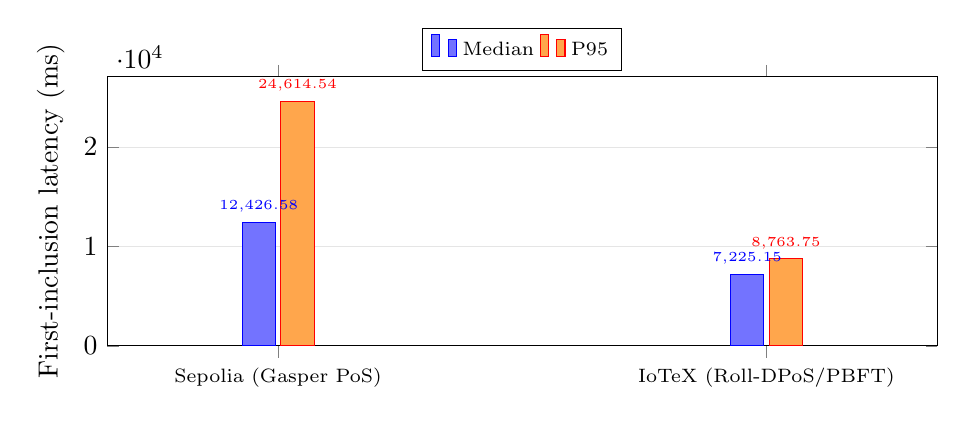
\begin{tikzpicture}
\begin{axis}[
  width=\columnwidth,height=5.0cm,ybar,bar width=12pt,
  ylabel={First-inclusion latency (ms)},
  symbolic x coords={Sepolia,IoTeX},xtick=data,
  xticklabels={Sepolia (Gasper PoS),IoTeX (Roll-DPoS/PBFT)},
  x tick label style={font=\scriptsize,align=center},
  legend style={at={(0.5,1.02)},anchor=south,legend columns=2,font=\scriptsize},
  ymin=0,nodes near coords,nodes near coords style={font=\tiny},
  enlarge x limits=0.35,ymajorgrids,grid style={black!10}
]
\addplot+[fill=blue!55] coordinates {(Sepolia,12426.58) (IoTeX,7225.15)};
\addplot+[fill=orange!70] coordinates {(Sepolia,24614.54) (IoTeX,8763.75)};
\legend{Median,P95}
\end{axis}
\end{tikzpicture}
\caption{Measured client-observed first-inclusion latency for matched,
concurrently submitted audit-anchor transactions. Public-testnet load and
RPC/client overhead are included; economic finality is not measured. Raft and
QBFT are compared structurally in Fig.~\ref{fig:consensus-protocols} but are
reported separately because their workloads and estimands are not comparable.}
\label{fig:pos-rolldpos-latency}
\end{figure}
